\subsection{综合图：完整模型、攻击预算与组件效应}
图\ref{fig:m-heat}--\ref{fig:m-component}展示完整网格。灰格表示未运行，误差棒为样本标准差；附录提供对应数值。
\begin{figure}[H]\centering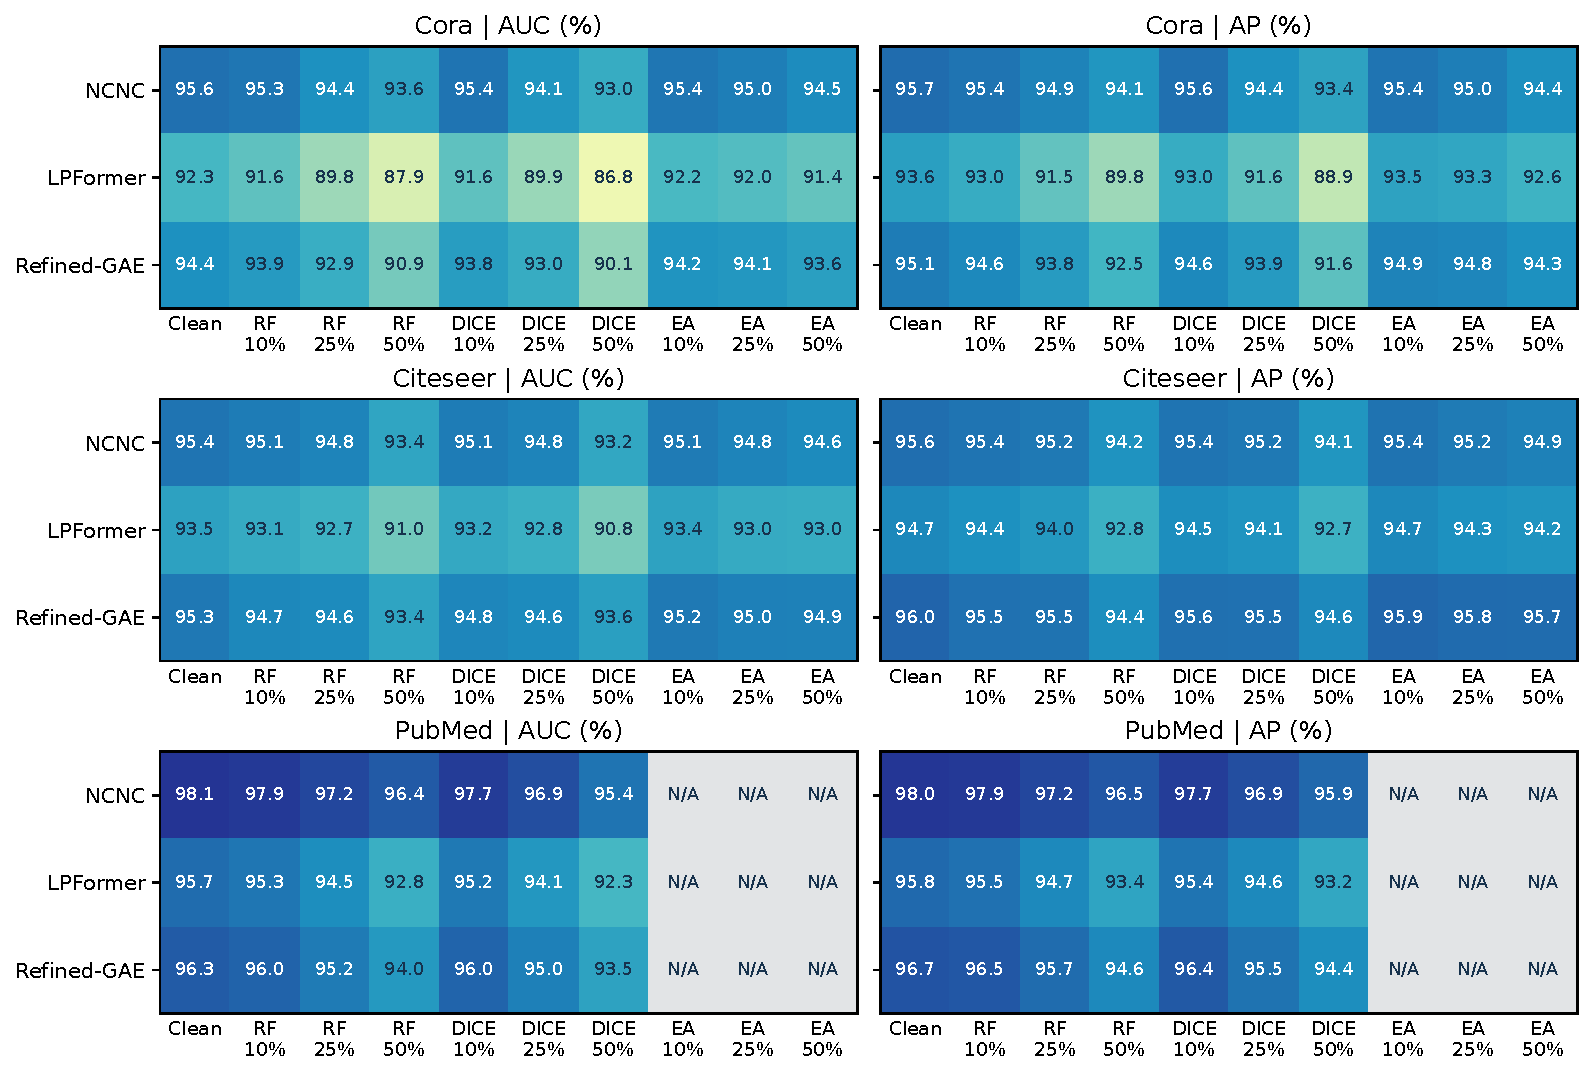
\includegraphics[width=23cm,height=11cm,keepaspectratio]{figures/main_full_models.pdf}\caption{M 协议：三个数据集完整模型的全部 AUC/AP 均值。PubMed EA 因节点上限跳过，其他 RF/DICE 三档及全部组件已运行。}\label{fig:m-heat}\end{figure}
\clearpage
\begin{figure}[H]\centering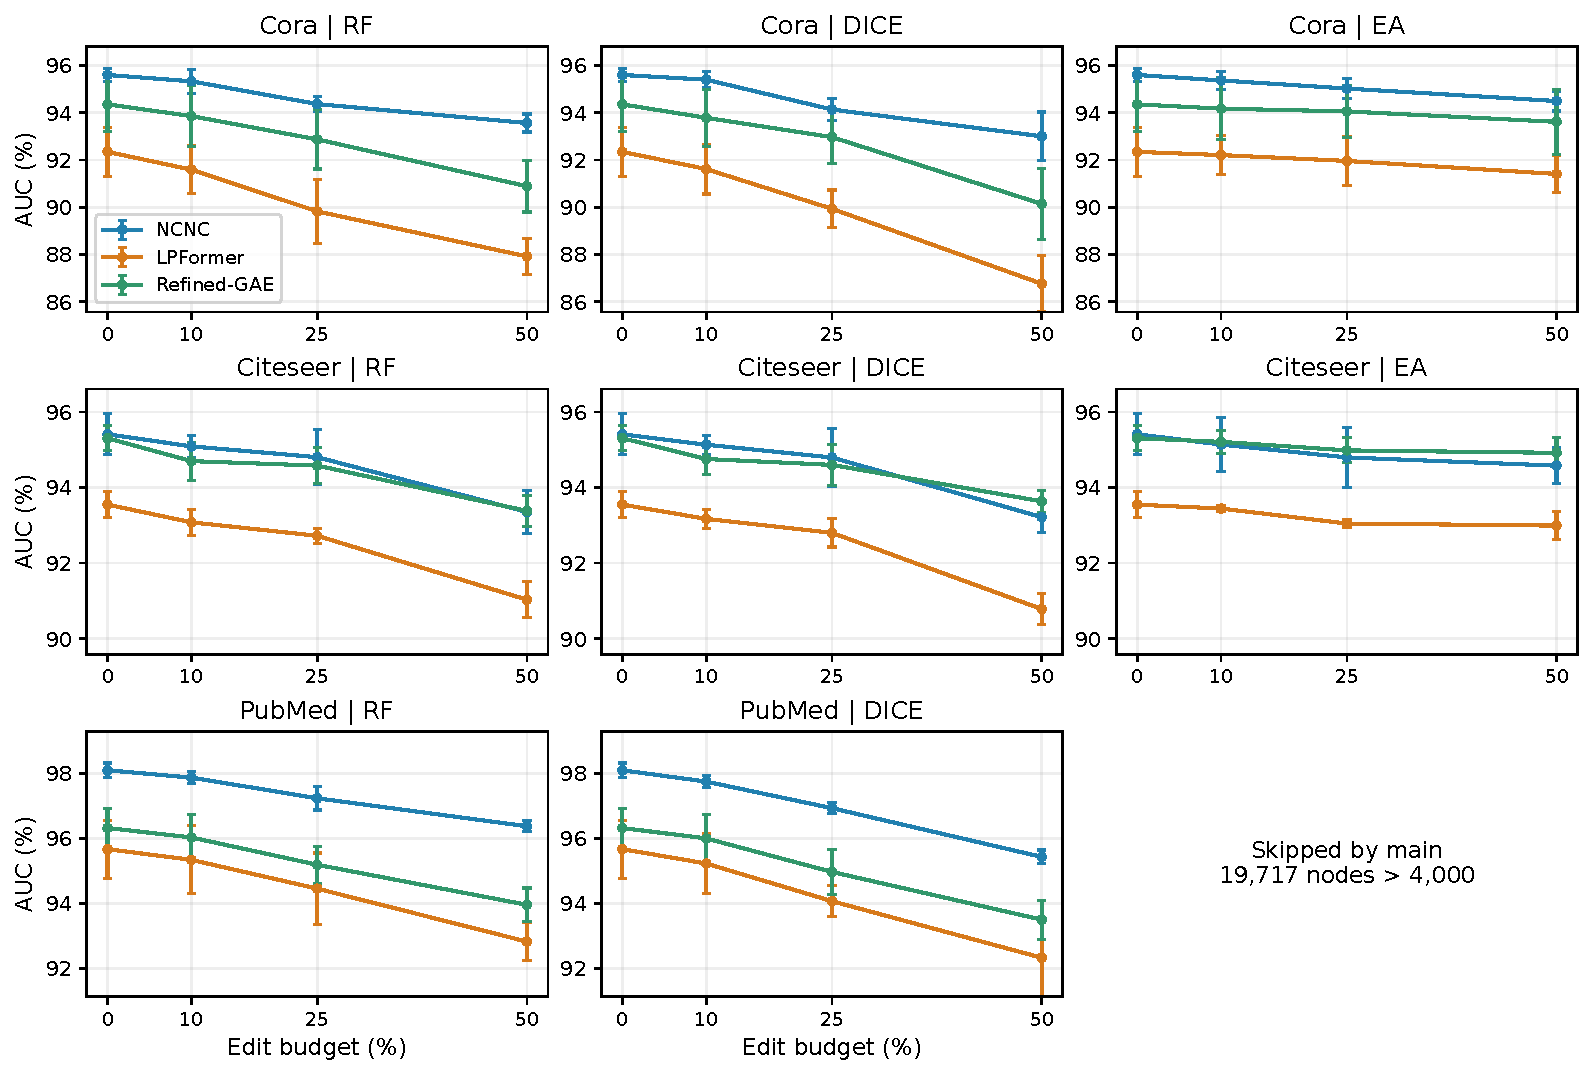
\includegraphics[width=23cm,height=14cm,keepaspectratio]{figures/main_attack_curves.pdf}\caption{M 协议：RF、DICE、EA 的预算曲线，均值与样本标准差。预算为完整图边数的混合编辑比例；不是纯删边比例。EA 的相对影响小只说明该代理攻击的迁移效果，不能推出对最强攻击安全。}\label{fig:m-curves}\end{figure}
\end{landscape}
\clearpage
\begin{figure}[H]\centering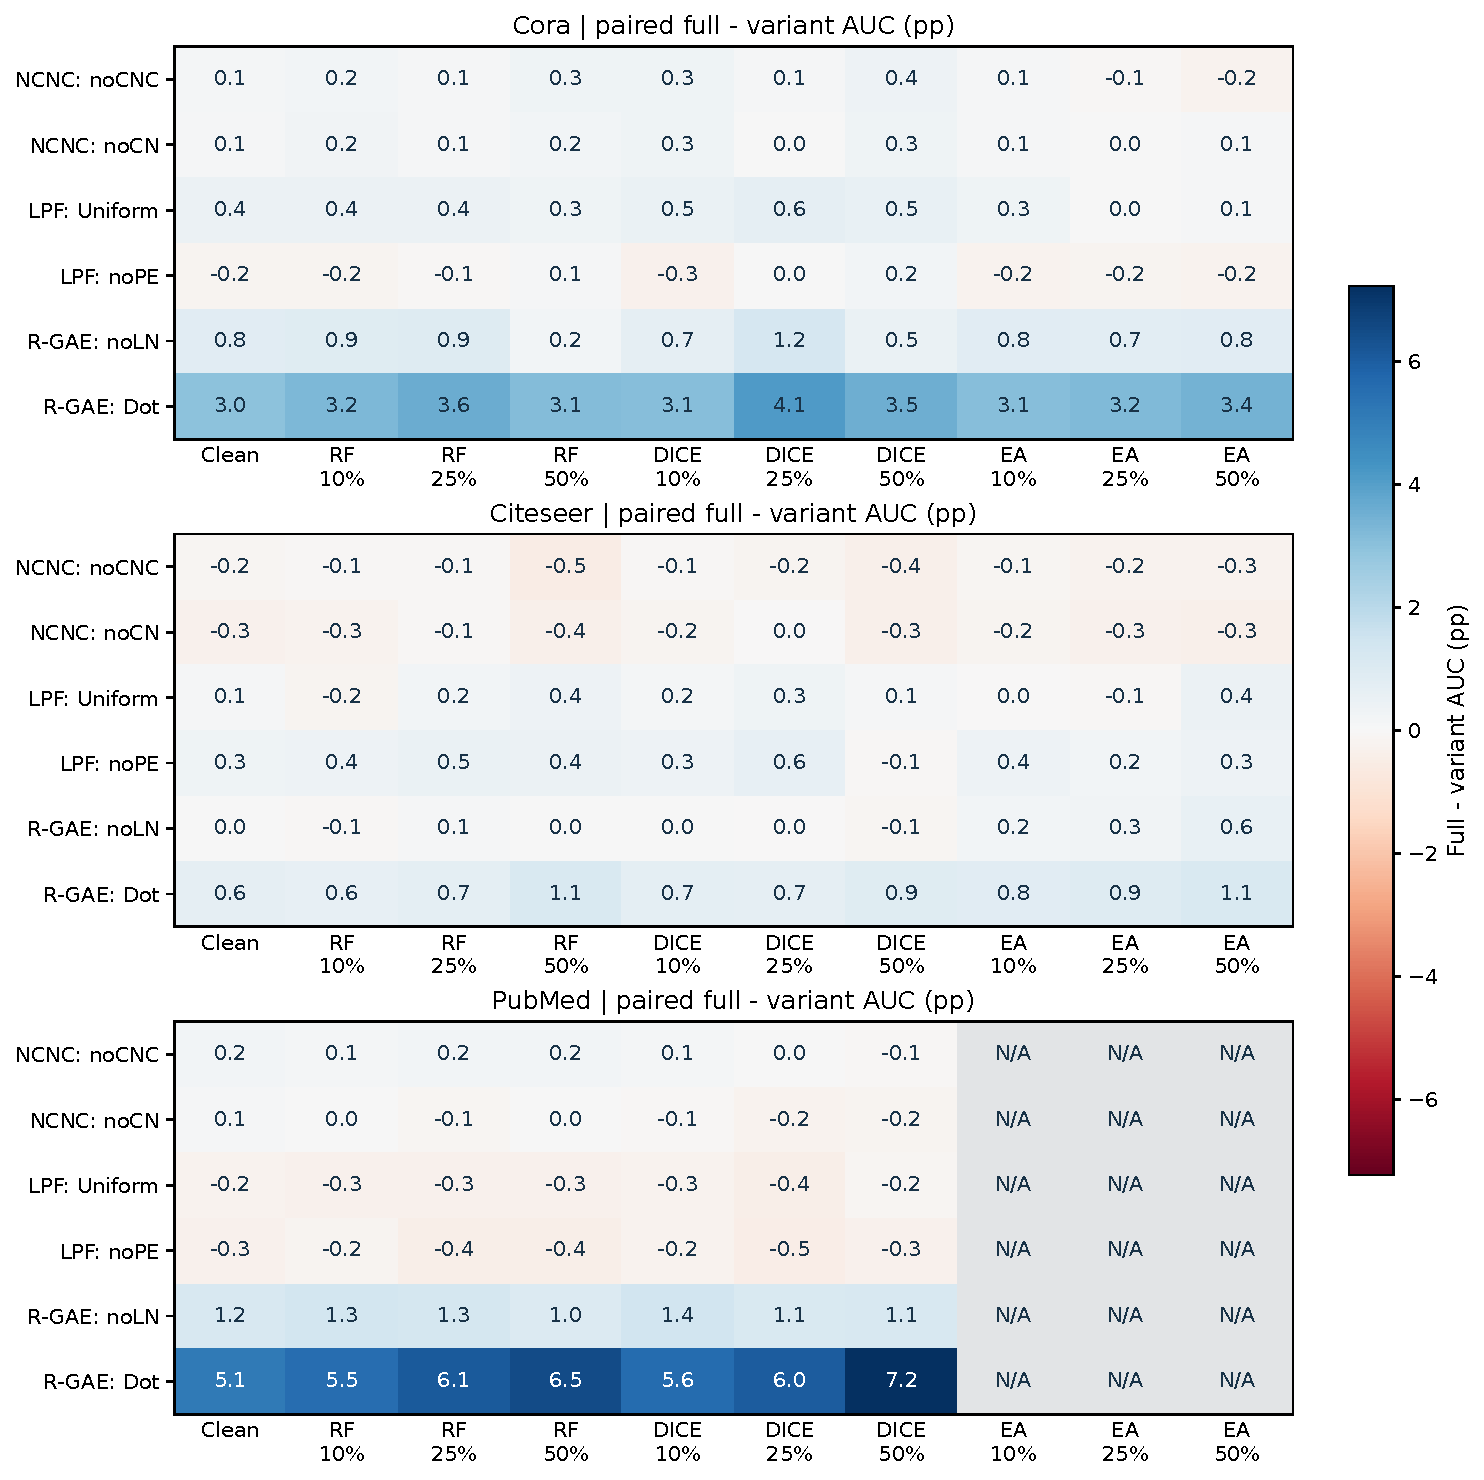
\includegraphics[width=\linewidth,height=.88\textheight,keepaspectratio]{figures/main_component_effects.pdf}\caption{M 协议：完整模型减去组件变体的配对 AUC（百分点）。正值为完整模型更高，负值为变体更高。每个变体独立重训；此图不是显著性检验。}\label{fig:m-component}\end{figure}
\clearpage
\subsection{完整模型：干净精度与攻击后精度}
{\small
\setlength{\tabcolsep}{3.2pt}
\renewcommand{\arraystretch}{1.10}
\begin{longtable}{llrrrr}
\caption{main 协议：完整模型 AUC（百分数）}\\
\toprule
数据 & 模型 & Clean & RF50 & DICE50 & EA50 \\
\midrule
\endfirsthead
\multicolumn{6}{l}{main 协议：完整模型 AUC（百分数）（续）}\\
\toprule
数据 & 模型 & Clean & RF50 & DICE50 & EA50 \\
\midrule
\endhead
\midrule\multicolumn{6}{r}{续下页}\\
\endfoot
\bottomrule
\endlastfoot
Cora & NCNC & $95.60\pm0.26$ & $93.57\pm0.38$ & $93.01\pm1.03$ & $94.50\pm0.42$ \\
Cora & LPFormer & $92.35\pm1.03$ & $87.92\pm0.76$ & $86.76\pm1.18$ & $91.41\pm0.79$ \\
Cora & Refined-GAE & $94.36\pm1.14$ & $90.89\pm1.09$ & $90.14\pm1.49$ & $93.62\pm1.37$ \\
Citeseer & NCNC & $95.41\pm0.54$ & $93.35\pm0.56$ & $93.22\pm0.40$ & $94.58\pm0.47$ \\
Citeseer & LPFormer & $93.55\pm0.35$ & $91.03\pm0.47$ & $90.78\pm0.42$ & $92.99\pm0.37$ \\
Citeseer & Refined-GAE & $95.31\pm0.33$ & $93.38\pm0.41$ & $93.64\pm0.29$ & $94.92\pm0.40$ \\
PubMed & NCNC & $98.09\pm0.22$ & $96.37\pm0.17$ & $95.43\pm0.21$ & N/A \\
PubMed & LPFormer & $95.66\pm0.89$ & $92.82\pm0.59$ & $92.32\pm1.22$ & N/A \\
PubMed & Refined-GAE & $96.32\pm0.61$ & $93.95\pm0.52$ & $93.50\pm0.60$ & N/A \\
\end{longtable}
}

\textbf{Cora。}NCNC 的干净 AUC 为 $95.60\pm0.26$，RF50、DICE50 后为 $93.57\pm0.38$、$93.01\pm1.03$，配对平均降幅2.03、2.60个百分点。LPFormer 对应降幅4.43、5.58，Refined-GAE为3.47、4.21。本次设置下，NCNC 在这两类扰动上同时具有较高攻击后均值与较小降幅；但此排名不是补全机制的因果证据，见后续消融。

\textbf{Citeseer。}干净均值为 NCNC95.41、Refined-GAE95.31、LPFormer93.55。DICE50 下 Refined-GAE 为 $93.64\pm0.29$，高于 NCNC 的 $93.22\pm0.40$；其平均降幅1.67也小于NCNC的2.19。EA50 下 Refined-GAE 为 $94.92\pm0.40$，也高于 NCNC 的 $94.58\pm0.47$。因此不能把 Cora 上的模型顺序概括成所有数据集通用的鲁棒性排名。

\textbf{PubMed。}NCNC 的干净、RF50、DICE50 AUC 分别为 $98.09\pm0.22$、$96.37\pm0.17$、$95.43\pm0.21$。LPFormer 对应为 $95.66\pm0.89$、$92.82\pm0.59$、$92.32\pm1.22$；Refined-GAE 为 $96.32\pm0.61$、$93.95\pm0.52$、$93.50\pm0.60$。NCNC 在该数据集这三条件均值最高。其 RF50/DICE50 平均降幅约1.72/2.67个百分点；LPFormer为2.84/3.34，Refined-GAE为2.36/2.82。所有三种子的原始值见附录，并未将三种子波动解释为统计显著性。

\textbf{攻击类型的解释。}Cora/Citeseer 中，EA50 的精度降幅通常小于 RF/DICE50。该现象只说明本次固定线性代理、删插配额、输入和采样下的迁移效果；代理目标可能与三个模型的薄弱点不一致。DICE 使用类别信息，因此也不能仅按降幅大小断言它是同信息预算下的最强攻击。

\subsection{配对消融：哪些机制受到数据支持}
{\footnotesize
\setlength{\tabcolsep}{3.2pt}
\renewcommand{\arraystretch}{1.10}
\begin{longtable}{lllrrrr}
\caption{M 协议组件效应：完整模型减变体 AUC（百分点）}\\
\toprule
数据 & 模型 & 变体 & Clean & RF50 & DICE50 & EA50 \\
\midrule
\endfirsthead
\multicolumn{7}{l}{M 协议组件效应：完整模型减变体 AUC（百分点）（续）}\\
\toprule
数据 & 模型 & 变体 & Clean & RF50 & DICE50 & EA50 \\
\midrule
\endhead
\midrule\multicolumn{7}{r}{续下页}\\
\endfoot
\bottomrule
\endlastfoot
Cora & NCNC & noCN & $0.09\pm0.51$ & $0.22\pm0.30$ & $0.32\pm0.71$ & $0.07\pm0.56$ \\
Cora & NCNC & noCNC & $0.14\pm0.52$ & $0.31\pm0.19$ & $0.37\pm0.51$ & $-0.25\pm0.25$ \\
Cora & LPFormer & noPE & $-0.21\pm0.56$ & $0.10\pm1.10$ & $0.21\pm1.16$ & $-0.23\pm0.38$ \\
Cora & LPFormer & Uniform & $0.43\pm1.23$ & $0.32\pm1.04$ & $0.52\pm1.30$ & $0.06\pm0.41$ \\
Cora & Refined-GAE & Dot & $2.98\pm0.98$ & $3.11\pm1.69$ & $3.52\pm1.95$ & $3.41\pm1.21$ \\
Cora & Refined-GAE & noLN & $0.80\pm0.79$ & $0.23\pm0.99$ & $0.47\pm1.24$ & $0.82\pm0.68$ \\
Citeseer & NCNC & noCN & $-0.31\pm0.32$ & $-0.39\pm0.22$ & $-0.35\pm0.33$ & $-0.35\pm0.10$ \\
Citeseer & NCNC & noCNC & $-0.15\pm0.35$ & $-0.51\pm0.19$ & $-0.38\pm0.50$ & $-0.25\pm0.17$ \\
Citeseer & LPFormer & noPE & $0.33\pm0.44$ & $0.45\pm0.57$ & $-0.07\pm0.18$ & $0.34\pm0.42$ \\
Citeseer & LPFormer & Uniform & $0.09\pm0.32$ & $0.37\pm0.31$ & $0.10\pm0.39$ & $0.44\pm0.43$ \\
Citeseer & Refined-GAE & Dot & $0.64\pm0.35$ & $1.13\pm0.52$ & $0.89\pm0.54$ & $1.11\pm0.60$ \\
Citeseer & Refined-GAE & noLN & $0.02\pm0.31$ & $0.04\pm0.64$ & $-0.14\pm0.58$ & $0.55\pm0.08$ \\
PubMed & NCNC & noCN & $0.07\pm0.36$ & $0.04\pm0.39$ & $-0.20\pm0.53$ & N/A \\
PubMed & NCNC & noCNC & $0.21\pm0.37$ & $0.21\pm0.29$ & $-0.11\pm0.44$ & N/A \\
PubMed & LPFormer & noPE & $-0.31\pm0.41$ & $-0.42\pm0.82$ & $-0.33\pm0.75$ & N/A \\
PubMed & LPFormer & Uniform & $-0.23\pm0.59$ & $-0.33\pm0.60$ & $-0.15\pm0.70$ & N/A \\
PubMed & Refined-GAE & Dot & $5.09\pm0.36$ & $6.47\pm0.94$ & $7.23\pm1.08$ & N/A \\
PubMed & Refined-GAE & noLN & $1.18\pm0.45$ & $0.98\pm0.69$ & $1.13\pm0.62$ & N/A \\
\end{longtable}
}

\textbf{NCNC：补全的边际收益较小且方向不稳定。}完整模型减 noCNC 的干净图差为 Cora $0.14\pm0.52$、Citeseer $-0.15\pm0.35$、PubMed $0.21\pm0.37$ 个百分点。完整模型的攻击表现不能直接归因于一次共同邻居补全。noCN 还保留结构传播，故其较小性能差不说明结构没有作用。当前结果更适合表述为：在作者超参数和统一训练预算下，端点编码分支已能保留相当一部分判别信息。

\textbf{LPFormer：学习注意力与位置编码并非稳定提升。}PubMed 上完整模型减 Uniform 的干净配对差为 $-0.23\pm0.59$，减 noPE 为 $-0.31\pm0.41$；DICE50 下完整减 noPE 为 $-0.33\pm0.75$。均值方向提示该设置中复杂组件未稳定带来收益，但三种子不能证明组件普遍无效。noPE 仍使用 PPR 筛选，不能以此推断模型不需要结构上下文。

\textbf{Refined-GAE：PubMed 的解码器选择影响较大。}完整模型减 Dot 的干净 AUC 为 $5.09\pm0.36$，DICE50 为 $7.23\pm1.08$ 个百分点。说明完整解码设计在本次 PubMed 设置下有明显的数值收益；该比较同时反映参数量、非线性、正则化及重新训练后的编码差异。它支持进一步检查点积几何表达的限制，不支持把全部差距归因于某个孤立的激活函数。

\subsection{与 main 已有 PubMed 结果的关系}
main 的 README、\code{docs/reproduction.md} 和 \code{results/sgdiff-paper-v2/} 已有 SGDiff PubMed 10种子结果，AUC 约 $0.902\pm0.002$，以及涉及 PubMed 的迁移记录。\code{configs/sgdiff_pubmed.yaml} 的1-hop、每跳20、结构扩散10步、特征64维两层/扩散50步、50训练轮和10预训练轮是 SGDiff 专属设置，不能套给这三个架构。

这些历史 SGDiff 结果与本文的种子数、候选规模、图缓存和训练配方不同。本文没有将 SGDiff 的0.902与三个新模型的均值作直接胜负比较，也没有用现有结果代替同图重跑。main 的 EA 节点上限是本次实现约束；原 SGDiff 论文包含 PubMed 鲁棒性表，二者必须区分。
